\documentclass[12pt]{beamer}
\usepackage[utf8]{inputenc}
\usepackage[german]{babel}
\usepackage{amsmath}
\usepackage{graphicx}
\usetheme{default}
\setbeamertemplate{footline}[frame number]
\begin{document}
	\author{Moritz Berger, Tim Herbermann,\\ Gerald Kolter, Sebastian Siebert}
	\title{Akustik}
	\subtitle{Grundpraktikum Teil I}
	%\logo{}
	%\institute{}
	%\date{}
	%\subject{}
	%\setbeamercovered{transparent}
	\setbeamertemplate{navigation symbols}{}
	\frame[plain]{\maketitle}
	
	\begin{frame}
		\frametitle{Einleitung}
		Seite 1
	\end{frame}

	\begin{frame}
		\frametitle{Schall \qquad Grundwissen}
		\begin{itemize}
		\item Schalldruck  $p(x, t) = p_0 cos(kt + \omega t)$
		\item Wellenzahl $k = 2\pi / \lambda$ und Kreisfrequenz $\omega = 2\pi f$
		\item Schallausbreitung mit $v = \frac{\Delta s}{\Delta t} = \lambda f$
		\end{itemize}
		\begin{itemize}
		\item test
		\end{itemize}
		
		
	\end{frame}

	\begin{frame}
		\frametitle{Laufzeitmessung \qquad Veruschsaufbau}
		\begin{center}
			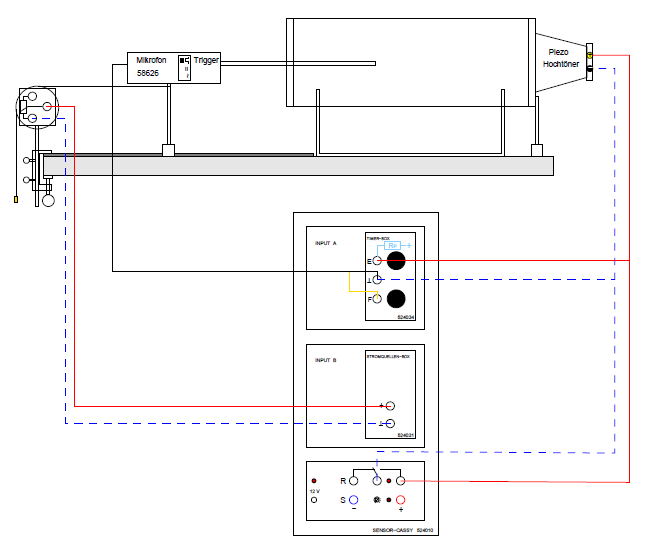
\includegraphics[width=0.8\linewidth]{aufbau_laufzeitmessung}
		\end{center}
	\end{frame}

	\begin{frame}
		\frametitle{Laufzeitmessung \qquad Rohdaten}
		\begin{center}
			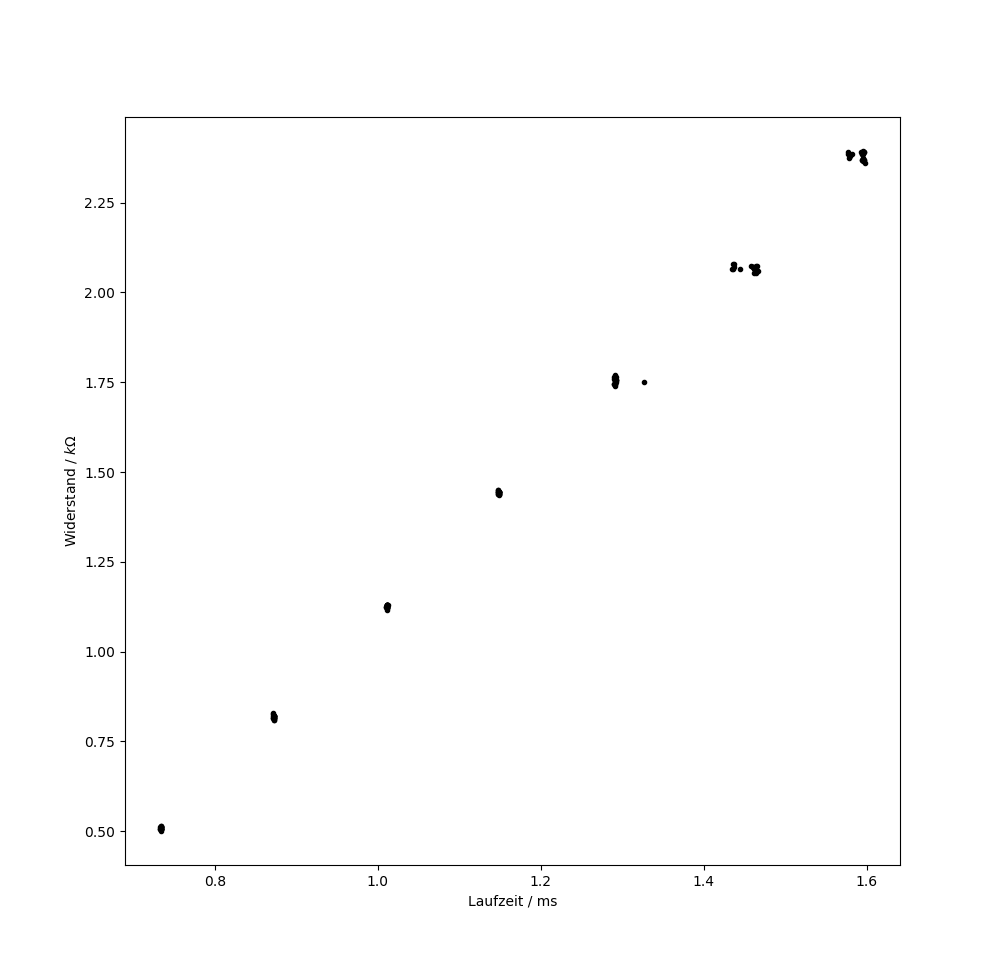
\includegraphics[width=0.8\linewidth]{rohdaten_laufzeit}
		\end{center}
	\end{frame}

	\begin{frame}
		\frametitle{Laufzeitmessung \qquad Auswertung}
		\begin{center}
			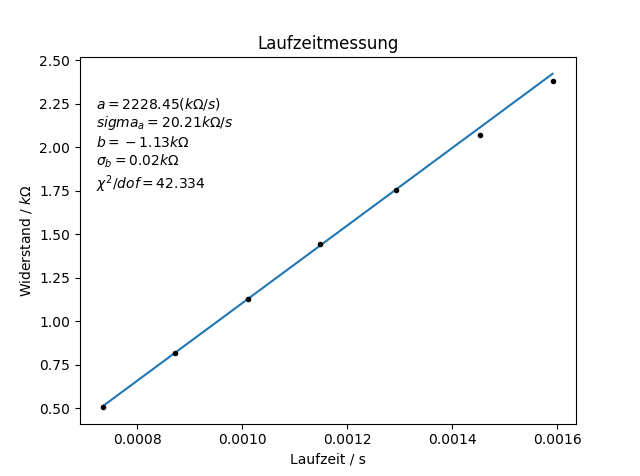
\includegraphics[width=0.6\linewidth]{fit_laufzeit}
		\end{center}
		\begin{itemize}
			\item Kalibration Poti: $\frac{\Delta s}{\Delta R} = (15,99 \pm 0,07) \frac{cm}{k\Omega}$\\ [0.3cm]
			\item Laufzeitmessung: $\frac{\Delta R}{\Delta t} = (2181,55 \pm 22,77) \frac{k\Omega}{s}$
		\end{itemize}
		$\Rightarrow v = \frac{\Delta s}{\Delta t} = (348,90 \pm 3,64 \pm 1,53) \frac{m}{s}$ \\ [0.3cm]
		\qquad $\sigma _{stat} = v \frac{\sigma _{\Delta R/\Delta t}}{\Delta R / \Delta t}$ \qquad $\sigma _{sys} = v \frac{\sigma _{\Delta s/\Delta R}}{\Delta s / \Delta R}$
	\end{frame}

	\begin{frame}
		\frametitle{Laufzeitmessung \qquad}
	\end{frame}
\end{document}